% !TEX TS-program = pdflatex
% !TEX encoding = UTF-8 Unicode

% This is a simple template for a LaTeX document using the "article" class.
% See "book", "report", "letter" for other types of document.

\documentclass[11pt]{article} % use larger type; default would be 10pt

\usepackage[utf8]{inputenc} % set input encoding (not needed with XeLaTeX)

%%% Examples of Article customizations
% These packages are optional, depending whether you want the features they provide.
% See the LaTeX Companion or other references for full information.

%%% PAGE DIMENSIONS
\usepackage{geometry} % to change the page dimensions
\geometry{a4paper} % or letterpaper (US) or a5paper or....
% \geometry{margin=2in} % for example, change the margins to 2 inches all round
% \geometry{landscape} % set up the page for landscape
%   read geometry.pdf for detailed page layout information

\usepackage{graphicx} % support the \includegraphics command and options

% \usepackage[parfill]{parskip} % Activate to begin paragraphs with an empty line rather than an indent

%%% PACKAGES
\usepackage{booktabs} % for much better looking tables
\usepackage{array} % for better arrays (eg matrices) in maths
\usepackage{amsfonts} % for maths fonts
\usepackage{amsmath} % for mathy text templates (propositions, theorems etc.)
\usepackage{amsthm} % proof env
\usepackage[hidelinks]{hyperref} % clickable, interactive references to equations, pages etc
\usepackage{paralist} % very flexible & customisable lists (eg. enumerate/itemize, etc.)
\usepackage{verbatim} % adds environment for commenting out blocks of text & for better verbatim
\usepackage{subfig} % make it possible to include more than one captioned figure/table in a single float
% These packages are all incorporated in the memoir class to one degree or another...

%%% HEADERS & FOOTERS
\usepackage{fancyhdr} % This should be set AFTER setting up the page geometry
\pagestyle{fancy} % options: empty , plain , fancy
\renewcommand{\headrulewidth}{0pt} % customise the layout...
\lhead{}\chead{}\rhead{}
\lfoot{}\cfoot{\thepage}\rfoot{}

%%% SECTION TITLE APPEARANCE
\usepackage{sectsty}
\allsectionsfont{\sffamily\mdseries\upshape} % (See the fntguide.pdf for font help)
% (This matches ConTeXt defaults)

%%% ToC (table of contents) APPEARANCE
\usepackage[nottoc,notlof,notlot]{tocbibind} % Put the bibliography in the ToC
\usepackage[titles,subfigure]{tocloft} % Alter the style of the Table of Contents
\renewcommand{\cftsecfont}{\rmfamily\mdseries\upshape}
\renewcommand{\cftsecpagefont}{\rmfamily\mdseries\upshape} % No bold!

%%% Math templates
\newtheorem{prop}{Proposition}
\newtheorem{lem}{Lemma}
\newtheorem{cor}{Corollary}
\newtheorem{thm}{Theorem}
\newtheorem{defn}{Definition}
\DeclareMathOperator*{\argmax}{arg\,max}

%%% END Article customizations

%%% The "real" document content comes below...

\title{An introduction to the mathematics of reinforcement learning theory}
\author{Sebastian Scherer}
%\date{} % Activate to display a given date or no date (if empty),
         % otherwise the current date is printed 

\begin{document}

\maketitle

\section{Preliminaries}

In reinforcement learning we concern ourselves with optimising the behaviour of an agent acting in a given environment to maximise some reward handed out by said environment. The agent's behaviour is governed by what we call control laws which act on the environment's current state, and can be probabilistic in nature. The environment responds to the agent's actions by assuming a new state and issuing a reward. The process of obtaining this new state and determining the value of said reward can also be probabilistic. In summary, our problem setting will be the (finite) repetition of the following steps:

\begin{enumerate}
	\item Determine current state $s_t$. For $t=0$ this will be a given starting state. For $t \ge 1$, this will be the environment probabilistically reacting to
	\begin{enumerate}
		\item The state $s_{t-1}$ in the previous time step.
		\item The action $a_{t-1}$ as chosen by the agent in the previous time step.
	\end{enumerate}
	\item Determine the agent's action $a_t$. This is done via the control law, which only considers the current state $s_t$, and nothing else, and is usually probabilistic.
	\item Based on $s_t$ and $a_t$, a probabilistic reward is handed out by the environment. For the last time step of the finite horizon problem, the reward only depends on $s_t$ since no further action will be taken.
\end{enumerate}

\subsection{The agent, the environment and the reward}\label{agentEnvironmentReward}

There are some constrains to this very general setting, which we will outline in this section. 

Firstly, we assume that at any time $t \in \mathbb{N}_0$, the environment can only assume one of finite states $s \in S$, where $S$ is the finite set of states possible. 

Similarly, we demand that our agent has only a finite set of actions $a \in A$, where $A$ is the finite set of actions, at his disposal at any given time $t \in \mathbb{N}_0$.

For an arbitrary but fixed starting state $s_0 \in S$, the continuous back-and-forth between the agent choosing an action $a_t$ and the environment assuming a subsequent state $s_{t+1}$ for $t=0,\dots,i$ (we ignore the rewards for the time being) leads to \textit{state-action trajectories} of the form

\begin{equation}\label{stateActionTraj}
	(s_0, a_0, s_1, a_1, \cdots, s_{i-1},a_{i-1},s_i,a_i).
\end{equation}

We will also sometimes refer to \textit{state trajectories}

\begin{equation}\label{stateActionTraj}
	(s_0, s_1, \cdots, s_{i-1},s_i,)
\end{equation}

 and \textit{action trajectories}

\begin{equation}\label{actionTraj}
	(a_0, a_1, \cdots, a_{i-1},a_i,)
\end{equation}

as needed. For any arbtrarily given but fixed end point in time $i \in \mathbb{N}_0$, we can imbue all of these three trajectory spaces with probability distributions depending on the control laws governing the actions (where plausible), and the probabilistic behaviour of the environment. We will do this in the next section.

The constraints on the environment's rewards are as follows. At any given time step $t$, the reward $r_t$ issued by the environment is distributed according to a distribution that only takes into account the present time step's state $s_t$ and agent action $a_t$. That is, the rewards awarded are instantaneous in nature and reward the current configuration of both agent and environment, but does not take into account the past. Furthermore, we assume that it is uniformly bounded, i.e. that 

\begin{equation}
	0 < r_t < M \,\, \forall t \in \mathbb{N}_0
\end{equation}

for some $M \in \mathbb{R}$. These considerations amount to the uniform boundedness of the conditioned expectations 

\begin{equation}
	0 < \mathbb{E}[r_t | s_t = s, a_t = a] =: R(a,s)_t < M
\end{equation}

for any $s \in S, a \in A$, $t \in \mathbb{N}_0$. We investigate these expectations more closely in the following section. For now, let it be mentioned that it is with respect to these, more precisely, trying to maximise these expected rewards, that we will try and optimise the control laws gouverning our agent's behaviour.

Lastly, we require our environment has no memory when evolving from one state to the next, be it in response to our agent's chosen action or otherwise. We demand that the environment's state at time $i+1$, $s_{i+1} \in S$, only depends on the previous time step's state, $s_i \in S$, and the agent's chosen action $a_i \in A$ at time $i$, but \textit{not} on any other preceding states and actions $s_t, a_t, t < i$ forming the state-action trajectory leading up to the state $s_i$ and action $a_i$ at time $i$. To be more precise, we require the \textit{transitional probabilities} of our environment to satisfy

\begin{equation}\label{transProbMarkov}
	Pr(s_{i+1} = s' | (s_0, a_0, \dots, s_i, a_i)) = Pr(s_{i+1} = s' | (s_i,a_i)) =: P^{a_i}_{s_i} (s')
\end{equation}

for all $s' \in S$ and $i \in \mathbb{N}_0$. This property is often referred to as the \textit{Markov} property.

\subsection{Probabilistic control laws}\label{probControlLaws}

In this section we will formalize our understanding of a \textit{control law}, which can be regarded as the decision making process of our agent at a fixed time $i \mathbb{N}_0$. A control law $\mu$ is a set of probability distributions over the action space $A$, one conditional distribution $\mu(s, \cdot)$ for each possible state $s \in S$. The idea is that, using the control law $\mu$ at time $i$ to make our agent's decision $a_i$, for any possible environment state $s$ $\mu$ generates a probability distribution over the action space $A$, assigning a probability

\begin{equation}\label{controlProb}
	\begin{array}{ll}
			& 	Pr(\text{Choosing action }a_i | \text{The environment is in state } s_i \text{ while following control law }\mu) \\
		=	&	Pr(\text{Choosing action }a_i | s_i, \mu) \\
		=:	&	\mu(s_i, a_i).
	\end{array}
\end{equation}

For completeness, we note that for any such control law $\mu$ clearly 

\begin{equation}\label{controlProbPositive}
	\mu(s,a) \ge 0
\end{equation}

 for every state action pair $(s,a) \in S \times A$, as well as 

\begin{equation}\label{controlProbSum1}
	\sum_{a \in A} \mu(s,a) = 1
\end{equation}

for all $s \in S$, must hold. 

It is worth noting that by the above interpretation we are only allowing control laws and distributions conditioned on \textit{only the immediate state} $s_i$, and nothing else. In this sense, the control laws considered have no memory of past environmental or agent behaviour either.

Before we conclude this section, let us develop a slightly more abstract but, as we shall see later, highly useful perspective on the set of control laws just outlined. We first order the finite state and action sets arbitrarily: $s^1,\dots,s^{|S|}$ and $a^1,\dots,a^{|A|}$. Since any control law $\mu$ is a collection of $|S|$ discrete probability distributions over $A$, we can identify $\mu$ with an element from $\mathbb{R}^{|S| \times |A|}$ via the canonical representation

\begin{equation}\label{controlProbMatrix}
	\mu = \left(	\begin{array}{cccc}
					\mu(s^1,a^1)	&	\mu(s^1,a^2)	&	\cdots 	&	\mu(s^1,a^{|A|}) \\
					\mu(s^2,a^1)	&	\mu(s^2,a^2)	&	\cdots 	&	\mu(s^2,a^{|A|}) \\
					\vdots 		&	\vdots 		& 	\ddots 	& 	\vdots \\
					\mu(s^{|S|},a^1)	&	\mu(s^{|S|},a^2)	&	\cdots 	&	\mu(s^{|S|},a^{|A|}) \\
				\end{array}
		\right).
\end{equation}

Here, the $i$-th row of the right hand side encodes the conditional probability distribution $\mu(s^i, \cdot)$ conditioned on state $s^i \in S$. We can thus see that the set of control laws can be identified with a closed and bounded, and therefore \textit{compact}, subset of the $\mathbb{R}^{|S| \times |A|}$ with its canonical norm via

\begin{equation}\label{defPolicySpace}
	\begin{array}{rcl}
		\Big\{ \mu | \mu \text{ is a control law} \Big\} 	& = & \Big\{ \mu \in \mathbb{R}^{|S| \times |A|} \Big| \mu_{ij} \ge 0 \, \forall i,j, \, \sum_{j=1}^{|A|} \mu_{ij} = 1 \, \forall i=1,\dots,|S| \Big\} \\
											& =: & \Pi(S,A).
	\end{array}
\end{equation}

The identification of the set of control laws with a compact set will be crucial in maximization arguments further down the line. Before that, however, let us next see how we can use these control laws to formalize the behaviour of our agent.

\subsection{Control law sequences and state-action trajectories}\label{controlLawTrajs}

In the previous section we have formalized the nature of our agent's decision making process at any given time $i$: Given that the environment is in state $s_i$ and our agent follows the control law $\mu$, it will pick any action $a \in A$ with probability $\mu(s_i,a)$. There is no reason for us to constrain our agent to keep using the same control law $\mu$ over time. It is much more desirable for our agent to be able to follow a sequence of different control laws, i.e. a \textit{policy}, say,

\begin{equation}\label{controlLawSeqence}
	\pi(i) = (\mu_0, \mu_1, \dots, \mu_i),
\end{equation}

where $\mu_t$ is the control law employed at time $t = 0,\dots i$ by our agent to pick action $a_i$. As referred to earlier, an environment with known transition probabilities $P^a_{ss'}, a \in A, s,s' \in S$ together with a policy $\pi(i)$ of control laws of length $i$ induces probability distributions on the sets of state-action, state and action trajectories. The environment's Markov property and the control laws' lack of memory allow for a nice factorization of these probabilities. The following Lemma makes this claim more precise.

\begin{figure}
  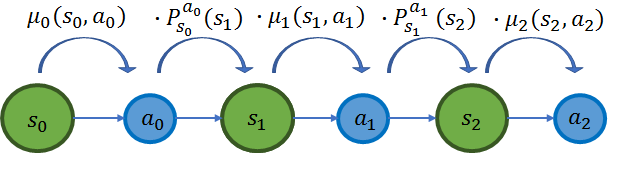
\includegraphics[width=\linewidth]{../graphics/state_action_probs.png}
  \caption{A trajectory starting from $s_0$ while following $\mu_0,\dots,\mu_i$ for $i = 2$}
  \label{fig:boat1}
\end{figure}

\begin{lem}{(State-action trajectory distribution under policies)}\label{lemStateActionControlLawTrajProb}

For some $i \in \mathbb{N}_0$, let $\pi(i)$ be a finite series of probabilistic control laws. Then for any fixed starting state $s_0 \in S$ and state-action trajectory $(s_0,a_0,\dots,s_i,a_i)$, the probability of obtaining said state-action trajectory up to time $i$ while following $\pi(i)$ is given by

\begin{equation}\label{stateActionControlLawTrajProb1}
	\prod_{t=0}^{i-1} \left( \mu_t(s_t,a_t) \cdot P^{a_t}_{s_t}(s_{t+1}) \right) \cdot \mu_i(s_i,a_i).
\end{equation}

\end{lem}

\begin{proof}

We prove this claim via induction over the control law sequence length parameter $i$. Since $i=0$ is somewhat trivial, we start our induction with $i=1$. We see that

\begin{equation}\label{controlLawTrajIA}
	\begin{array}{ll}
			& \Pr\{(s_0,a_0, s_1, a_1) | \text{ starting at } s_0 \text{ and following } \pi(1) = (\mu_0,\mu_1)\} \\
		=	& \Pr\{(s_0,a_0, s_1, a_1) | s_0, \, \pi(1)\} = \Pr\{(s_0,a_0) \cap (s_1,a_1) | s_0, \, \pi(1)\} \\
		=	& \Pr\{(s_0,a_0, s_1) | s_0, \, \pi(1)\} \cdot \Pr\{a_1 |(s_0,a_0,s_1), \, s_0, \, \pi(1)\} \\
		=	& \Pr\{(s_0,a_0,s_1) | s_0, \, \mu_0\} \cdot \Pr\{a_1 | s_1, \, \mu_1)\} \\
		=	& \Pr\{(s_0,a_0) | s_0, \, \mu_0\} \cdot \Pr\{s_1 | (s_0,a_0), \, \mu_0 \} \cdot \Pr\{a_1 | s_1, \, \mu_1)\} \\
		=	& \mu_0(s_0,a_0) \cdot \, P^{a_0}_{s_0}(s_1) \cdot \mu_1(s_1,a_1). \\
	\end{array}
\end{equation}

Now assume this claim holds for some $i-1 \in \mathbb{N}_0$. The exact same argument applied above then yields

\begin{equation}\label{controlLawTrajIS}
	\begin{array}{ll}
			& \Pr\{(s_0,a_0,\dots, s_i, a_i) | \text{ starting at } s_0 \text{ and following } \pi(i)\} \\
		=	& \Pr\{(s_0,a_0,\dots, s_i, a_i) | s_0, \, \pi(i)\} \\
		=	& \Pr\{(s_0,a_0,\dots, s_{i-1}, a_{i-1}) \cap (s_i,a_i) | s_0, \, \pi(i)\} \\
		=	& \Pr\{(s_0,a_0,\dots, s_{i-1}, a_{i-1},s_i) | s_0, \, \pi(i)\} \cdot \Pr\{a_i |(s_0,a_0,\dots, s_{i-1}, a_{i-1},s_i), \, s_0, \, \pi(i)\} \\
		=	& \Pr\{(s_0,a_0,\dots, s_{i-1}, a_{i-1},s_i) | s_0, \, \pi(i-1)\} \cdot \Pr\{a_i | s_i, \, \mu_i)\} \\
		=	& \Pr\{(s_0,a_0,\dots, s_{i-1}, a_{i-1}) | s_0, \, \pi(i-1)\} \\
			& \cdot \Pr\{s_i | (s_0,a_0,\dots, s_{i-1}, a_{i-1}), \, s_0, \, \pi(i-1) \} \cdot \Pr\{a_i | s_i, \, \mu_i)\} \\
		=	& \Pr\{(s_0,a_0,\dots, s_{i-1}, a_{i-1}) | s_0, \, \pi(i-1)\} \\
			& \cdot \Pr\{s_i | (s_{i-1}, a_{i-1}) \} \cdot \Pr\{a_i | s_i, \, \mu_i)\} \\
		=	& \Pr\{(s_0,a_0,\dots, s_{i-1}, a_{i-1}) | s_0, \, \pi(i-1)\} \cdot P^{a_{i-1}}_{s_{i-1}}(s_i) \cdot \mu_i(s_i,a_i) \\
		=	& \prod_{t=0}^{i-2} \left( \mu_t(s_t,a_t) \cdot P^{a_t}_{s_t}(s_{t+1}) \right) \cdot \mu_{i-1}(s_{i-1,}a_{i-1}) \cdot P^{a_{i-1}}_{s_{i-1}}(s_i) \cdot \mu_i(s_i,a_i) \\		
		=	& \prod_{t=0}^{i-1} \left( \mu_t(s_t,a_t) \cdot P^{a_t}_{s_t}(s_{t+1}) \right) \cdot \mu_i(s_i,a_i).
	\end{array}
\end{equation}

\end{proof}

Similarly, without executing the last action at time $t = i$ and thus effectively only following $\pi(i-1) = (\mu_0,\dots,\mu_{i-1})$ we obtain the corollary result

\begin{cor}(State-action trajectory distribution under policies II)\label{corStateActionControlLawTrajProb1}

For some $i \in \mathbb{N}_0$, let $\pi(i-1)$ be a finite series of probabilistic control laws. Then for any fixed starting state $s_0 \in S$ and state-action trajectory $(s_0,a_0,\dots,s_i)$, the probability of obtaining said state-action trajectory up to time $i-1$ while following $\pi(i-1)$ is given by

\begin{equation}\label{stateActionControlLawTrajProb2}
	\prod_{t=0}^{i-1} \left( \mu_t(s_t,a_t) \cdot P^{a_t}_{s_t}(s_{t+1}) \right).
\end{equation}

\end{cor}

Given a some starting state $s_0$, what about the chances of following \textit{any} state-action trajectory ending with some specified state-action pair $(s_i,a_i) \in S \times A$? Clearly, the answer is to simply add over all relevant state-action trajectory probabilities.

\begin{cor}(State-action trajectory distribution under policies III)\label{corStateActionControlLawTrajProb2}

For some $i \in \mathbb{N}_0$, let $\pi(i)$ be a finite series of probabilistic control laws, and let $(s,a) \in S \times A$ be any fixed but arbitrary state-action pair.Let finally $s_0 = s' \in S$ be some fixed but arbitrary starting state. Then the probability of following \textit{any} of the state-action trajectories $(s',a_0,...,s,a)$, $a_t \in A$ for $t=0,...,i-1$, $s_t \in S$ for $t=1,...,i-1$, while following $\pi(i)$ is given by

\begin{equation}\label{stateActionControlLawTrajProb3}
	\sum_{\begin{array}{c}
			s_0 = s' \\
			a_0,\dots,a_{i-1} \in A \\
			s_1,\dots,s_{i-1} \in S
		\end{array}}\Big[ \prod_{t=0}^{i-2} \left( \mu_t(s_t,a_t) \cdot P^{a_t}_{s_t}(s_{t+1}) \right) \cdot \mu_{i-1}(s_{i-1},a_{i-1}) \cdot P^{a_{i-1}}_{s_{i-1}}(s) \Big] \cdot \mu_i(s,a).
\end{equation}

\end{cor}

\begin{proof}

Using Lemma \ref{lemStateActionControlLawTrajProb}, we immediately arrive at the expression in Eq. \ref{stateActionControlLawTrajProb3} by summing over the set of relevant trajectories.

\begin{equation}\label{}
	Tr_{s'}^{s,a} =  \left\{(s',a_0,s_1,a_1,\dots,s_{i-1},a_{i-1},s,a) \Bigg| \begin{array}{lr}
															a_0, \dots, a_{i-1} \in A, \\
															s_1,\dots,s_{i-1} \in S
													\end{array} \right\}.
\end{equation}

\end{proof}

\begin{figure}
  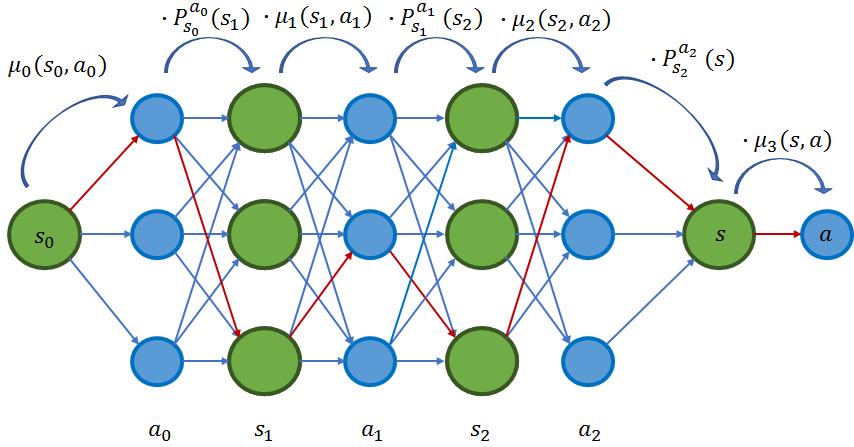
\includegraphics[width=\linewidth,height=8cm]{../graphics/state_action_probs_2.png}
  \caption{All the possible trajectories $(s_0,\dots,s,a)$ starting from $s_0$ while following $\mu_0,\dots,\mu_i$ for $i = 3$, $|S| = |A| = 3$. A sample trajectory is highlighted in magenta.}
  \label{fig:boat1}
\end{figure}

Before we turn to the rewards in the next section, let us view this section's results from a functional point of view.

In our theoretical considerations, we usually assume the environment's transitional probabilities $P^a_{ss'}, a \in A, s,s' \in S$ to be both constant and known. Since the finding of a policy that is in some way optimal will be our main goal, it is intuitive to view all formulae derived in Lemma \ref{}, Corollary \ref and Corollary \ref{} as functions of some policy $\pi = (\mu_0,\dots,\mu_i)$. Recollecting our embedding of individual policies $\mu$ into (subsets) of $\mathbb{R}^{|S| \times |A|}$ in section \ref{}, Eq. \ref{defPolicySpace}, we can see that the space of all policies of length $i$ can be seen as

\begin{equation}
	\begin{array}{rcl}
		\Big\{ \pi(i) | \pi(i) \text{ is a policy of length } i+1 \Big\} & = & \Big\{ \pi(i) = (\mu_t)_{t=0,\dots,i} \Big| \mu_t \textit{ is a control law } \Big\} \\
		& \cong & \Pi(S,A)^{i+1},
	\end{array}
\end{equation}

the three aforementioned results induce 3 continuous (the control laws' matrix representations' coefficients are being added and multiplied only - continuous operations) functions on the \textit{compact} set $\Pi(S,A)^i$. We spell this out explicitly for the most important result, Corollary \ref{corStateActionControlLawTrajProb2}.

\begin{cor}\label{corContProbMap}
	Let $s' \in S$ be a fixed but arbitrary starting state, and let $i \in \mathbb{N}_0$. Let further $(s,a) \in S \times A$ be a fixed but arbitrary state-action pair. Then the function

\begin{equation}\label{contProbMap}
	\begin{array}{rccl}
		p_{s'}(s,a,i): 	& \Pi(S,A)^i 			& \rightarrow 	& [0,1] \\
					& (\mu_t)_{t=0,\dots,i} 	& \mapsto 	& \Pr\left\{  (s',a_0,\dots,s,a), \, \Bigg| \begin{array}{lr}
																					a_0, \dots, a_{i-1} \in A, \\
																					s_1,\dots,s_{i-1} \in S, \\
																					\pi(i)
																					\end{array} \right\}
	\end{array}
\end{equation}

mapping policies onto their conditional probabilities of following \textit{any} trajectory ending in $(s,a)$, conditioned on starting at $s_0$, is continuous on the space of permissable policies.
\end{cor}

\begin{proof}
	The proof consists solely in realizing that, for any policy $\pi(i) = (\mu_0,\dots,\mu_i) \in \Pi(S,A)^i$, the image of $\pi(i)$ under $p_{s'}(s,a)$ is of course the expression appearing in \ref{stateActionControlLawTrajProb3}, where $s_0$ understood to be fixed at $s'$. This in turn is merely a sum of products of all of the guiding policy $\pi(i)$'s components' coefficients, and hence continuous in $\pi(i) \in \Pi(S,A)^i$, endowed with its canonical $| \cdot |_{\mathbb{R}^i}$ norm.
\end{proof}

A direct consequence of this is that for any choice of starting state $s'$ and ending state-action pair $(s,a) \in S \times A$, the function $p_{s'}(s,a)$ as defined in \ref{contProbMap} attains its maximum over the space of permissable policies of length $\Pi(S,A)^i$.

\subsection{Rewards revisited}

We have gathered enough preliminary results to return to a closer inspection our main object of focus: the rewards issued by the environment, depending on the state-action trajectories along which our agent travels.

Recall that at any time step $t$, we are given the immediate reward $r_t$'s expectation conditioned only $s_t$ and $a_t$ (i.e. ignoring \textit{all} previous elements of the state-action trajectory) as

\begin{equation}
	\mathbb{E}[r_t | (s_0,a_0,\dots,s_{t-1},a_{t-1},s,a)] = \mathbb{E}[r_t | s_t = s, a_t = a] =: R(s,a)_t.
\end{equation}

If we are interested in the expectation of $r_t$ at time $t$ in \textit{general}, i.e. without conditioning on $s_t$ and $a_t$, can use the above to see that generally

\begin{equation}\label{eqExpReward}
	\begin{array}{rcl}
		\mathbb{E}[r_t]	& = &	\sum_r \Pr\{r_t = r\} \cdot r \\
					& = & 	\sum_r \left(\sum_{a \in A} \sum_{s \in S} \Pr\{r_t = r | s_t = s, a_t = a\} \cdot \Pr\{ a_t = a \cap s_t = s \} \right) \cdot r \\
					& = &	\sum_{a \in A} \sum_{s \in S} \Pr \{a_t = a \cap s_t = s\} \sum_r \Pr \{r_t = r | a_t = a, s_t = s\} \cdot r \\
					& = &	\sum_{a \in A} \sum_{s \in S} \Pr \{a_t = a \cap s_t = s\} \cdot \mathbb{E}[r_t | a_t = a, s_t = s] \\
					& = &	\sum_{a \in A} \sum_{s \in S} \Pr \{a_t = a \cap s_t = s\} \cdot R(s,a)_t \\
	\end{array}
\end{equation}

It is natural to ask about the rather generic expression $\Pr(a_t = a \cap s_t = s)$ appearing in the above equation and how it might be connected to the control law sequences we discussed in the previous section. What Eq. \ref{eqExpReward} tells us is that obtaining the expectation of $r_t$ requires the knowledge of the probability of observing the state action pair $(s,a)$ at $t$ for \textit{all} $s \in S, a \in A$. This in turn implies that for any finite policy $\pi(i) = (\mu_0,\dots,\mu_i)$, $i \ge t$, and starting state $s'$, we must have 

\begin{equation}\label{eqExpReward}
	\begin{array}{rcl}
		\mathbb{E}[r_t | s_0 = s', \pi(i)]	& = &	\sum_{a \in A} \sum_{s \in S} \Pr \{a_t = a \cap s_t = s | s_0 = s', \pi(i)\} \cdot R(s,a)_t \\
								& = &	\sum_{a \in A} \sum_{s \in S} p_s'(s,a,t) \cdot R(s,a)_t \\
	\end{array}
\end{equation}

Our knowledge of $p_s'(s,a)$ then ensures that the mapping

\begin{equation}\label{contExpRewMap}
	\begin{array}{rccl}
		\mathbb{E}[r_t | s_0 = s', \pi(i)]: 	& \Pi(S,A)^i 	& \rightarrow 	& [0,M] \\
									& \pi(i)				 		& \mapsto 	& \sum_{a \in A} \sum_{s \in S} p_s'(s,a,t) \cdot R(s,a)_t
	\end{array}
\end{equation}

is continuous as a finite sum of continuous functions for any $s' \in S$, provided $i \ge t$. This result is worth repeating in cursive.

\begin{cor}{(Continuity of policy induced rewards w.r.t guiding policy)}\label{corContinuousReward}
For each $t \in \mathbb{N}_0$, $i \ge t$, and starting state $s' \in S$, the reward $r_t$'s expectation $\mathbb{E}[r_t | s' = s_0, \pi(i)]$, taken over all trajectories starting at $s'$ and sampled according to some $\pi(i) \in \Pi(S,A)^i$, depends continuously on the guiding policy $\pi(i)$. As such, it attains its maximum on $\Pi(S,A)^i$.
\end{cor}

\section{The discounted finite horizon problem}

We dedicate this section to the formulation and solution of the so-called discounted finite horizon problem. We will use the results obtained in this section to solve the infinite horizon counterpart problem later.

Let $0 < \gamma < 1$,$s' \in S$ a fixed but arbitrary starting state, and let $i \in \mathbb{N}$ be given. The discounted finite horizon problem is the searching of a policy $\pi$ as discussed in section \ref{} that, conditioned on starting at $s'$ at $t=0$, maximizes the induced finite sum of discounted expected rewards. To be more precise, putting

\begin{equation}\label{eqFinDiscHorReward}
		J(s',\pi(i)) := \sum_{t=0}^i \mathbb{E}[ \gamma^t \cdot r_t | s_0 = s', \pi(i)] = \sum_{t=0}^i \gamma^t \cdot \mathbb{E}[ r_t | s_0 = s', \pi(i)],
\end{equation}

our discounted finite horizon problem reduces to, given an arbitrary but fixed starting state $s' \in S$, finding

\begin{equation}\label{eqFinDiscHorProb}
	\pi(i)^* := \argmax_{\pi(i) \in \Pi(S,A)^i} J(s',\pi(i)).
\end{equation}

The existence of a solution to problem \ref{eqFinDiscHorProb} follows more or less directly from our previous work.

\begin{prop}(Existence of a solution)\label{lemExistenceFiniteSolution}
	For any $i \in \mathbb{N}_0$, $s' \in S$, the discounted finite horizon problem has a solution in $\Pi(S,A)^{i+1}$.
\end{prop}

\begin{proof}
By Corollary \ref{corContinuousReward}, the mapping 

\begin{equation}\label{contDiscExpRewSumMap}
	\begin{array}{rccl}
		J(s',\cdot): 	& \Pi(S,A)^{i+1} 	& \rightarrow 	& [0,i M] \\
					& \pi(i)		& \mapsto 	& \sum_{t=0}^i \gamma^t \cdot \mathbb{E}[ r_t | s_0 = s', \pi(i)]
	\end{array}
\end{equation}

is continuous as the sum of continuous functions, and therefore attains its maximum at some $\pi(i)^*$ in the compact normed space $(\Pi(S,A)^i,|\cdot|_{\mathbb{R}^i})$.
\end{proof}

From now on, we will denote the solution of the discounted finite horizon problem by $\pi(i)$, and we will denote the maximum discounted cumulative reward achieved by this solution as 

\begin{equation}
	J^*(s') := J(s',\pi(i)^*) = \max_{\pi(i) \in \Pi(S,A)^i} J(s',\pi(i))
\end{equation}

Making use of some auxiliary results from calculus layed out in the appendix, we can do better and give a more constructive approach. Informally speaking, the solution to \ref{eqFinDiscHorProb} can be obtained by 'rolling the reward up from the back'. This is formalized in the following

\begin{prop}(Building of a solution)\label{lemBuildingFiniteSolution}
	Consider the discounted finite horizon problem as defined in \ref{eqFinDiscHorProb}. Set
\begin{equation}
	\begin{array}{rllr}
		\hat{J}_{-1,i}(s') & = & 0 \\
		\hat{J}_{j,i}(s') & := & \max_{\mu_{i-j} \in \Pi(S,A)} \left( \mathbb{E}\left[r_{i-j} + \hat{J}_{j-1,i}(s') \bigg| \begin{array}{c}
																							s_0 = s', \\
																							(\mu_0,\dots,\mu_{i-j})
																						\end{array} 
																							\right] \right), & j=0,\dots,i, \\
	
		\mu^*_{i-j} & := & \argmax_{\mu_{i-j} \in \Pi(S,A)} \left( \mathbb{E}\left[r_{i-j} + \hat{J}_{j-1,i}(s')  \bigg| \begin{array}{c}
																							s_0 = s', \\
																							(\mu_0,\dots,\mu_{i-j})
																						\end{array} 
																							\right] \right), & j=0,\dots,i. \\
	\end{array}
\end{equation}

Then

\begin{equation}
	J^*(s') = \hat{J}_{i,i}(s')
\end{equation}

and

\begin{equation}
	\pi(i)^* = (\mu^*_0,\dots,\mu^*_i).
\end{equation}

\end{prop}

One detail that might not be immediately obvious but is worth noting is that the expression $\hat{J}_{j,i}(s')$, $j=0,\dots,i$ is still very much dependent on the yet-to-be fixated control laws $\mu_0,\dots,\mu_{i-j-1}$ that help induce the underlying trajectories' distribution. Essentially, we are taking a continuous function ($J(s',\cdot)$) of multiple variables ($\mu_0,\dots,\mu_i \in \Pi(S,A)$, respectively) and maximize one dimension at a time, starting with the 'last' one, $\mu_i$, to obtain the function's global maximum over the entire domain ($\Pi(S,A)^{i+1}$).

\end{document}